\documentclass[10pt]{exam}
% подключаем кириллицу 
\usepackage[T2A]{fontenc}
\usepackage[utf8]{inputenc}

\usepackage[margin=0.7in]{geometry}
\usepackage{amsmath,amssymb}
\usepackage{multicol}
\usepackage{graphicx}
\usepackage{pbox}

\newcommand{\class}{Информатика I}
\newcommand{\term}{Весна 2016}
\newcommand{\examnum}{Экзамен 1}
\newcommand{\examdate}{4/2/2016}
\newcommand{\timelimit}{120 Минут}

\pagestyle{head}
\firstpageheader{}{}{}
\runningheader{\class}{\examnum\ - Страница № \thepage\ из \numpages}{\examdate}
\runningheadrule

\pointname{ баллов}
\vqword{Вопрос}
\vpword{Баллы}
\vsword{Набранные баллы}
\vtword{Всего:}

\begin{document}

\noindent
\begin{tabular*}{\textwidth}{l @{\extracolsep{\fill}} r @{\extracolsep{6pt}} l}
\textbf{\class} & \textbf{Имя Фамилия:} & \makebox[2in]{\hrulefill}\\
\textbf{\term} &&\\
\textbf{\examnum} &&\\
\textbf{\examdate} &&\\
\textbf{Длительность: \timelimit} &  & 
\end{tabular*}\\
\rule[2ex]{\textwidth}{2pt}

\numpages\ страниц (включая эту) и \numquestions\ вопросов.
Общее число баллов \numpoints.


\begin{center}
Таблица баллов (заполняется преподавателем)\\
\addpoints
\gradetable[v][questions]
\end{center}

\noindent
\rule[2ex]{\textwidth}{2pt}

\newpage
\begin{questions}

\section{Вопросы}
\vbox{
\question[10] Чему равен порядок роста продолжительности работы следующего участка кода:
\begin{verbatim}
int sum = 0;
for (int i = 0; i < N; i++)
    for (int j = i+1; j < N; j++)
        for (int k = j+1; k < N; k++)
            for (int h = 0; h < N; h++)
                sum++;
\end{verbatim}

\begin{checkboxes}
\choice $O(1)$
\choice $O(n)$
\choice $O(n^3)$
\choice $O(n^3 \sqrt{n})$
\choice $O(n^3 \log{n})$
\choice $O(n^4)$
\end{checkboxes}
}

\vbox{
\question[20] Расположите следующие функции в порядке увеличения скорости роста:
\begin{multicols}{3}
\begin{choices}
\choice $\log{n}$
\choice $1$
\choice $e^n$
\choice $n$
\choice $\log{\log{n}}$
\choice $n\sqrt{n}$
\choice $n!$
\choice $n^n$
\choice $n\log{n}$
\choice $n^2$
\choice $2^n$
\end{choices} 
\end{multicols}
\makeemptybox{1in}
}

\vbox{
\checkboxchar{$\Box$} % changing checkbox style locally
\question[20] Отметьте все функции, чьё O-большое равно $O(n^2)$
\begin{multicols}{2}
\begin{checkboxes}
\choice $1000 n^2$
\choice $1$
\choice $e^n$
\choice $4 n^2 + 10 n + 50$
\choice $n^3 + 100 n^2$
\choice $n^3 - 100 n^2$
\choice $n\log{n}$
\choice $n^3 / (1 + n)$
\end{checkboxes}
\end{multicols}
}


\vbox{%
\checkboxchar{$\Box$} % changing checkbox style locally
\question[20] Какие утверждения об алгоритмах сортировки верны (можно отметить несколько вариантов).
\addpoints
\begin{checkboxes}
\choice Если мы не знаем никакой дополнительной информации об элементах массива, то оптимальная сложность сортировки числового массива равна $O(n \log{n})$
\choice Есть только один алгоритм сортировки, имеющий оптимальную сложность.
\choice Алгоритм быстрой сортировки основан на принципе "разделяй и властвуй"
\choice Время работы большинства алгоритмов сортировки не зависит от расположения элементов во входном массиве
\end{checkboxes}
}


\vbox{%
\question[10] Пусть у уже отсортированного массива длины $N$ переставили $k$  раз соседние элементы (например, 100-й элемент переставили с 101-ым, 242-й с 243-й, так $k$ перестановок). При этом известно, что $k \ll N$. Какой из алгоритмов будет лучшим выбором для сортировки такого массива.
\addpoints
\begin{checkboxes}
\choice Сортировка выбором
\choice Сортировка вставками
\choice Сортировка пузырьком
\choice Сортировка слиянием
\choice Быстрая сортировка
\end{checkboxes}
}

\question[20] Пусть есть массив чисел: \;
42 55 34 11 41 97 44 20 47 65 \\
Найдите массив, который получится после применения 4-х шагов(замен) сортировки выбором.
\makeemptybox{1in}


\vbox{
\question[25] Заполните таблицу:
\addpoints
\begin{center}
  \begin{tabular}{ l || c }
    \hline
    Алгоритм & Сложность(в среднем) \\ \hline \hline
    Сортировка пузырьком & $O(n^2)$  \\ \hline
    Сортировка вставками &   \\ \hline
    Сортировка слиянием &   \\ \hline
    Быстрая сортировка &   \\ \hline
    Сортировка выбором & \\ \hline
    Простейший алгоритм перемножения матриц nxn & \\ \hline
    Простейший алгоритм сложения матриц nxn & \\ \hline
  \end{tabular}
\end{center}
}

\vbox{
\question[25] Заполните таблицу:
\addpoints
\begin{center}
  \begin{tabular}{ l || c | c }
    \hline
     & Доступ к элементу & Вставка элемента \\ \hline \hline
    Массив &  &  \\ \hline
    Односвязный список(list) &  &  \\ \hline
    Двоичное дерево поиска &  &  \\ \hline
    Хеш-таблица & $O(1)$ & $O(1)$ \\ \hline
  \end{tabular}
\end{center}
}

\vbox{
\checkboxchar{$\Box$}
\question[15] Отметьте все преимущества односвязного списка по сравнению со статическим массивом.
\addpoints
\begin{checkboxes}
\choice Односвязный список занимает меньше памяти, чем массив
\choice В односвязном списке можно гораздо быстрее найти нужный элемент
\choice В односвязный список можно гораздо быстрее добавлять элемент
\choice В односвязный список можно добавлять и удалять элементы динамически(т.е. во время работы программы).
\choice Все элементы односвязного списка хранятся в памяти локально(друг за другом), что иногда может быть полезно.
\end{checkboxes}
}


\vbox{
\question[10] Класс NP это:
\addpoints
\begin{checkboxes}
\choice Класс задач, которые можно за полиномиальное время решить на\\ детерминированной машине Тьюринга.
\choice Класс задач, которые можно за полиномиальное время решить на\\ недетерминированной машине Тьюринга.
\choice Класс алгоритмов, которые можно за полиномиальное время решить на детерминированной машине Тьюринга.
\choice Класс алгоритмов, которые можно за полиномиальное время решить на недетерминированной машине Тьюринга.
\end{checkboxes}
}

\vbox{
\question[10] Как соотносятся между собой классы P и NP?
\addpoints
\begin{multicols}{2}
\begin{choices}
\choice \includegraphics[width=0.3\textwidth]{images/pnp1.png}  
\choice \includegraphics[width=0.3\textwidth]{images/pnp2.png}  
\choice \includegraphics[width=0.2\textwidth]{images/pnp3.png}  
\choice \includegraphics[width=0.2\textwidth]{images/pnp4.png}  
\end{choices}
\end{multicols}
Если сомневаетесь в выборе варианта, можете дать развёрнутый ответ:
\makeemptybox{1in}
}



\vbox{
\question[30] Пусть на вход алгоритма построения бинарного дерева поиска поступает следующая последовательность: 91 40 22 87 36 60 27 43 62 24 \\
Постройте получившиеся бинарное дерево поиска.
\addpoints
\makeemptybox{4in}
Предположим, что вам потребовалось найти в этом дереве число 76. Найдите последовательность чисел, с которыми число 76 будет сравниваться.
\makeemptybox{0.5in}
}



\question[55] Рассмотрим следующий взвешенный ориентированный граф: \\
\includegraphics[width=0.4\textwidth]{images/graph_empty.png} \\
11.A. (5 баллов) Найдите число вершин и рёбер данного графа.
\makeemptybox{0.3in}
\vbox{
11.Б. (15 баллов) Известно, что есть 2 стандартных представления графа: список смежных вершин и матрица смежности. Представьте данный граф в обоих представлениях.
\makeemptybox{2.0in}
}
\vbox{
11.В. (35 баллов) Пошагово проиллюстрируйте работу алгоритма Дейкстры на этом графе.
\begin{multicols}{2}
1)\includegraphics[width=0.4\textwidth]{images/graph.png} \hfill
2)\includegraphics[width=0.4\textwidth]{images/graph_empty.png} \hfill
3)\includegraphics[width=0.4\textwidth]{images/graph_empty.png} \hfill
4)\includegraphics[width=0.4\textwidth]{images/graph_empty.png} \hfill
\vfill
5)\includegraphics[width=0.4\textwidth]{images/graph_empty.png} \hfill
6)\includegraphics[width=0.4\textwidth]{images/graph_empty.png} \hfill
7)\includegraphics[width=0.4\textwidth]{images/graph_empty.png} \hfill
8)\includegraphics[width=0.4\textwidth]{images/graph_empty.png} \hfill
\end{multicols} 
}




\section{Задачи на программирование}
\vbox{
\question[80] Алгоритм бинарного поиска -- это алгоритм поиска элемента в отсортированном массиве, использующий дробление массива на половины.\\
На вход алгоритма подаётся отсортированный по возрастанию массив и число, которое требуется в нём найти. Поиск осуществляется путём сравнения числа, которое нужно найти, с центральным элементом массива. Если это число оказалось больше центрального элемента, то оно рекурсивно ищется в правой половине массива, а если меньше, то в левой.
\addpoints
}

\vbox{
\question[150] Реализуйте алгоритм волновой трассировки.\\

\begin{multicols}{2}
\pbox{12cm}{
\includegraphics[width=0.38\textwidth]{images/lee.png} \\ \\
  \begin{tabular}{ l || l }
    \hline
    Вход & Выход \\ \hline
    \pbox{12cm}{
    4 5\\
    0 0 1 0 0 \\
    0 0 1 0 0 \\
    0 0 1 0 0 \\
    0 0 0 0 0 \\
    2 0 \\
    0 3
    }
    &
    \pbox{12cm}{
    (2, 0) -> (2, 1) -> \\
    (3, 1) -> (3, 2) -> \\
    (3, 3) -> (2, 3) -> \\
    (1, 3) -> (0, 3) 
    }
  \end{tabular}
  }
  \\

От стартовой ячейки порождается шаг в соседнюю ячейку, при этом проверяется, проходима ли она, и не принадлежит ли ранее меченной в пути ячейке. При выполнении условий проходимости и непринадлежности её к ранее помеченным в пути ячейкам, в атрибут ячейки записывается число, равное количеству шагов от стартовой ячейки, от стартовой ячейки на первом шаге это будет 1. Каждая ячейка, меченая числом шагов от стартовой ячейки становится стартовой и из неё порождаются очередные шаги в соседние ячейки. 
Восстановление кратчайшего пути происходит в обратном направлении: при выборе ячейки от финишной ячейки к стартовой на каждом шаге выбирается ячейка, имеющая атрибут расстояния от стартовой на единицу меньше текущей ячейки. 
\end{multicols}
Считывание входа и построение графа (35 баллов из 125)\\
Распространение волны (35 баллов из 125):
\begin{verbatim}
ЦИКЛ
  ДЛЯ каждой ячейки loc, помеченной числом d
    пометить все соседние свободные непомеченные ячейки числом d + 1
  КЦ
  d := d + 1
ПОКА (финишная ячейка не помечена) И (есть возможность распространения волны) 
\end{verbatim}
Восстановление пути (55 баллов из 125):
\begin{verbatim}
ЕСЛИ финишная ячейка помечена
ТО
  перейти в финишную ячейку
  ЦИКЛ
    выбрать среди соседних ячейку, помеченную числом на 1 меньше числа в текущей ячейке
    перейти в выбранную ячейку и добавить её к пути
  ПОКА текущая ячейка — не стартовая
  ВОЗВРАТ путь найден
ИНАЧЕ
  ВОЗВРАТ путь не найден
\end{verbatim}

}


\end{questions}

\end{document}
